
\documentclass[11pt]{article}

% --------------------------------------------------
% Packages
% --------------------------------------------------
\usepackage[T1]{fontenc}
\usepackage[utf8]{inputenc}
\usepackage{lmodern}
\usepackage{amsmath,amssymb,amsthm,mathtools}
\usepackage{geometry}
\usepackage{hyperref}
\usepackage{enumitem}
\usepackage{microtype}
\usepackage{graphicx}
\usepackage[nameinlink,noabbrev]{cleveref}
\usepackage{verbatim}
\geometry{margin=1in}
\hypersetup{colorlinks=true,linkcolor=blue,citecolor=blue,urlcolor=blue}

% --------------------------------------------------
% Theorem environments
% --------------------------------------------------
\newtheorem{theorem}{Theorem}[section]
\newtheorem{definition}[theorem]{Definition}
\newtheorem{lemma}[theorem]{Lemma}
\newtheorem{axiom}[theorem]{Axiom}
\newtheorem{remark}[theorem]{Remark}
\newtheorem{corollary}[theorem]{Corollary}
\newtheorem{proposition}[theorem]{Proposition}

% --------------------------------------------------
% Macros
% --------------------------------------------------
\newcommand{\Coh}{\mathbf{Coh}}
\newcommand{\Hom}{\mathrm{Hom}}
\newcommand{\id}{\mathrm{id}}
\newcommand{\ACCEPT}{\mathrm{ACCEPT}}
\newcommand{\REJECT}{\mathrm{REJECT}}
\newcommand{\RV}{\mathrm{RV}}
\newcommand{\syn}{\mathrm{syn}}
\newcommand{\semc}{\mathrm{sem}}
\newcommand{\Qbar}{\overline{\mathbb Q}_{\ge 0}}
\newcommand{\Kadm}{\mathcal{K}}
\newcommand{\Hid}{\mathcal{H}}
\newcommand{\F}{\mathcal{F}}
\newcommand{\Rset}{\mathcal{R}}
\newcommand{\Trace}{\mathsf{Trace}}
\newcommand{\Payload}{\mathsf{Payload}}
\newcommand{\Tok}{\mathsf{Tok}}
\newcommand{\Hist}{\mathsf{Hist}}
\newcommand{\Pfin}{\mathcal{P}_{\mathrm{fin}}}

% --------------------------------------------------
% Title
% --------------------------------------------------
\title{\textbf{The Coh Category:\\
Verifier-Certified Trace Composition and Projection-Induced Semantic Cost}}
\author{NoeticanLabs Research Division}
\date{\today}

\begin{document}
\maketitle

\begin{abstract}
We define the Coh category, a verifier-indexed categorical structure in which morphisms are generated by admissibility rather than assumed a priori. A Coh system consists of observable states, hidden-state realizations, a proposal mechanism, an exact rational valuation, and a deterministic verifier.

Morphisms are finite certified traces satisfying both verifier acceptance and a resource inequality. We prove that these certified traces form a category under concatenation. We then distinguish syntactic bookkeeping cost from semantic cost derived from hidden realizations, and prove a projection-induced subadditive semantic cost law.

A worked example exhibits a strict separation between syntactic and semantic cost, showing that projection can destroy enough hidden information that realized cost is strictly smaller than visible bookkeeping. The result is a precise categorical framework for verifier-certified execution traces in resource-constrained computation.
\end{abstract}

\section{Introduction}

In many formal systems, composition is treated as primitive and legality as secondary. In verification-sensitive computation, the order should be reversed: a transition should count as a morphism only after it has survived certification.

The central claim of this paper is therefore:
\[
\boxed{
\text{Morphisms are verifier-certified traces, not raw arrows.}
}
\]

This distinguishes the present framework from weighted or resource-aware categories in which morphisms are typically given first and only later decorated with costs; compare the classical enrichment perspective of Kelly \cite{kelly1982} and the quantitative viewpoint of Lawvere \cite{lawvere1973}. In the Coh framework, admissibility generates morphisms.

The scope of the paper is deliberately narrow. We do \emph{not} claim a universal computation substrate. Instead, we isolate a foundational verification wedge: a category of certified execution traces with exact rational bookkeeping and a distinct semantic cost law induced by projection from hidden realizations.

The paper makes four concrete contributions:
\begin{itemize}[leftmargin=2em]
\item We define a verifier-indexed category whose morphisms are admissible traces.
\item We prove categorical closure under trace concatenation.
\item We distinguish syntactic bookkeeping cost from semantic cost and prove a projection-induced subadditive semantic cost law.
\item We give a worked example in which semantic cost is strictly smaller than syntactic cost.
\end{itemize}

\begin{figure}[t]
\centering
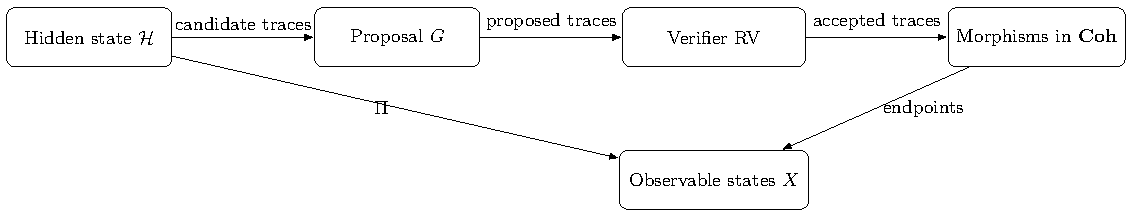
\includegraphics[width=0.9\textwidth]{../figures/architecture.pdf}
\caption{Coh execution wedge. Hidden-state proposals generate candidate traces, the verifier certifies a subset, and only certified traces enter the categorical layer. Projection to observables induces a semantic cost law distinct from syntactic bookkeeping.}
\label{fig:architecture}
\end{figure}

\section{Preliminaries: exact numerics, payloads, and traces}

\begin{definition}[Exact nonnegative extended rationals]
Define
\[
\Qbar := \mathbb Q_{\ge 0}\cup\{+\infty\}.
\]
The foundational valuation layer of the paper takes values in $\Qbar$, while all stepwise bookkeeping quantities take values in $\mathbb Q_{\ge 0}$.
\end{definition}

\begin{definition}[Typed payloads and compiled control tokens]
Let $X$ be a set of observable states. For each ordered pair $(x,y)\in X\times X$, let
\[
\Payload(x,y)
\]
be a payload type of semantic meaning objects carried by transitions from $x$ to $y$.

Let $\Tok$ be a set of control tokens, and for each $(x,y)$ let
\[
\kappa_{x,y}:\Payload(x,y)\to \Tok
\]
be a compilation map from payloads to control tokens.
\end{definition}

\begin{definition}[Primitive step]
A primitive step $\sigma:x\leadsto y$ consists of:
\begin{itemize}[leftmargin=2em]
\item source and target states $x,y\in X$,
\item a payload $p_\sigma\in \Payload(x,y)$,
\item a compiled token $\kappa_{x,y}(p_\sigma)\in \Tok$,
\item exact rational bookkeeping data
\[
s(\sigma),d(\sigma)\in \mathbb Q_{\ge 0},
\]
\item a well-typedness obligation certifying that the payload is meaningful at $(x,y)$ and compiles to the designated token.
\end{itemize}
\end{definition}

\begin{definition}[Finite traces]
Let $\Trace(X)$ denote the set of finite composable sequences of primitive steps over $X$. A trace
\[
\tau:x\rightsquigarrow y
\]
is written
\[
x=x_0 \xrightarrow{\sigma_1} x_1 \xrightarrow{\sigma_2}\cdots \xrightarrow{\sigma_n} x_n=y.
\]
\end{definition}

\begin{definition}[Syntactic bookkeeping]
For a trace $\tau$, define its syntactic spend and syntactic defect by
\[
s_{\syn}(\tau):=\sum_{i=1}^n s(\sigma_i),
\qquad
d_{\syn}(\tau):=\sum_{i=1}^n d(\sigma_i).
\]
\end{definition}

\begin{definition}[Concatenation]
If $\tau_1:x\rightsquigarrow y$ and $\tau_2:y\rightsquigarrow z$, define the concatenation
\[
\tau_2 * \tau_1 : x\rightsquigarrow z
\]
by appending the step-sequence of $\tau_2$ after that of $\tau_1$.
\end{definition}

\section{Coh systems}

\begin{definition}[Coh system]
A Coh system is a tuple
\[
\mathcal S=(X,\Kadm,\Hid,\Pi,\Hist,V,G,\RV)
\]
where:
\begin{itemize}[leftmargin=2em]
\item $X$ is an observable state space,
\item $\Kadm\subseteq X$ is the admissible subset,
\item $\Hid$ is a hidden-state space,
\item $\Pi:\Hid\to X$ is the projection to observable state,
\item $\Hist$ is a history/context type,
\item $V:X\to \Qbar$ is a valuation,
\item $G:\Hid\times \Hist\to \Pfin(\Trace(X))$ is a proposal mechanism,
\item $\RV:\Hid\times \Trace(X)\times \Hid\times \Hist\to\{\ACCEPT,\REJECT\}$ is a deterministic verifier.
\end{itemize}
\end{definition}

\begin{definition}[Finite-valued admissible states]
The admissible subset $\Kadm$ satisfies
\[
x\in \Kadm \Longrightarrow V(x)\in \mathbb Q_{\ge 0}.
\]
Equivalently,
\[
\Kadm \subseteq \{x\in X: V(x)<+\infty\}.
\]
\end{definition}

\begin{definition}[Hidden fibers]
For $x\in X$, define the fiber
\[
\F_x:=\{\Psi\in\Hid:\Pi(\Psi)=x\}.
\]
\end{definition}

\begin{remark}
There is exactly one hidden layer in the theory, namely $\Hid$. All hidden representatives are elements of $\Hid$, and all observable states arise by projection through $\Pi$.
\end{remark}

\section{Admissible traces}

\begin{definition}[Admissible trace]
A trace $\tau:x\rightsquigarrow y$ is \emph{admissible} if:
\begin{enumerate}[label=(\roman*),leftmargin=2em]
\item $x,y\in\Kadm$,
\item there exist hidden representatives
\[
\Psi_x\in\F_x,\qquad \Psi_y\in\F_y,
\]
and a history
\[
H\in\Hist
\]
such that
\[
\tau\in G(\Psi_x,H),
\qquad
\RV(\Psi_x,\tau,\Psi_y,H)=\ACCEPT,
\]
\item the resource inequality holds in $\mathbb Q_{\ge 0}$:
\[
V(y)+s_{\syn}(\tau)\le V(x)+d_{\syn}(\tau).
\]
\end{enumerate}
\end{definition}

\section{Verifier axioms}

\begin{axiom}[Identity acceptance]
For every $x\in\Kadm$, every $\Psi_x\in\F_x$, and every admissible history $H\in\Hist$, the empty trace
\[
\epsilon_x:x\rightsquigarrow x
\]
satisfies
\[
\epsilon_x\in G(\Psi_x,H),
\qquad
\RV(\Psi_x,\epsilon_x,\Psi_x,H)=\ACCEPT.
\]
\end{axiom}

\begin{axiom}[Verifier closure under concatenation]
Suppose
\[
\tau_1\in G(\Psi_x,H_1),\qquad \RV(\Psi_x,\tau_1,\Psi_y,H_1)=\ACCEPT,
\]
and
\[
\tau_2\in G(\Psi_y,H_2),\qquad \RV(\Psi_y,\tau_2,\Psi_z,H_2)=\ACCEPT.
\]
Then there exists a compatible history $H_{12}\in\Hist$ such that
\[
\tau_2 * \tau_1 \in G(\Psi_x,H_{12}),
\qquad
\RV(\Psi_x,\tau_2 * \tau_1,\Psi_z,H_{12})=\ACCEPT.
\]
\end{axiom}

\begin{axiom}[Separation law]
Syntactic spend and syntactic defect are distinct and non-interchangeable:
\[
s_{\syn}(\tau)\not\equiv d_{\syn}(\tau).
\]
\end{axiom}

\section{The Coh category}

\begin{definition}[Hom-set]
For $x,y\in\Kadm$, define
\[
\Hom_{\Coh(\mathcal S)}(x,y)
:=
\{\tau:x\rightsquigarrow y \mid \tau \text{ is admissible}\}.
\]
\end{definition}

\begin{definition}[Identity morphism]
For each $x\in\Kadm$, define
\[
\id_x:=\epsilon_x.
\]
\end{definition}

\begin{definition}[Composition]
Given
\[
\tau_1\in\Hom(x,y),\qquad \tau_2\in\Hom(y,z),
\]
define
\[
\tau_2\circ \tau_1:=\tau_2 * \tau_1.
\]
\end{definition}

\begin{lemma}[Identity admissibility]\label{lem:id-adm}
For each $x\in\Kadm$, $\id_x\in \Hom(x,x)$.
\end{lemma}

\begin{proof}
By Identity Acceptance, the empty trace $\epsilon_x$ is verifier-accepted and proposed. Since $x\in\Kadm$, the valuation $V(x)$ is finite rational. Also,
\[
s_{\syn}(\epsilon_x)=0,\qquad d_{\syn}(\epsilon_x)=0,
\]
so the resource inequality reads
\[
V(x)+0\le V(x)+0,
\]
which holds. Thus $\epsilon_x$ is admissible.
\end{proof}

\begin{lemma}[Closure under composition]\label{lem:comp-adm}
If
\[
\tau_1\in\Hom(x,y),\qquad \tau_2\in\Hom(y,z),
\]
then
\[
\tau_2\circ \tau_1 \in \Hom(x,z).
\]
\end{lemma}

\begin{proof}
Since $\tau_1,\tau_2$ are admissible, we have
\[
x,y,z\in\Kadm.
\]
Hence
\[
V(x),V(y),V(z)\in \mathbb Q_{\ge 0}
\]
by finite-valued admissibility.

Verifier acceptance of the composite follows from the verifier closure axiom.

For the resource inequality, admissibility gives
\[
V(y)+s_{\syn}(\tau_1)\le V(x)+d_{\syn}(\tau_1),
\]
\[
V(z)+s_{\syn}(\tau_2)\le V(y)+d_{\syn}(\tau_2).
\]
These are inequalities in $\mathbb Q_{\ge 0}$, so ordinary addition is valid. Adding them yields
\[
V(y)+V(z)+s_{\syn}(\tau_1)+s_{\syn}(\tau_2)
\le
V(x)+V(y)+d_{\syn}(\tau_1)+d_{\syn}(\tau_2).
\]
Since $V(y)$ is finite, we may cancel it from both sides and obtain
\[
V(z)+s_{\syn}(\tau_1)+s_{\syn}(\tau_2)
\le
V(x)+d_{\syn}(\tau_1)+d_{\syn}(\tau_2).
\]
Because syntactic bookkeeping is additive under concatenation,
\[
s_{\syn}(\tau_2 * \tau_1)=s_{\syn}(\tau_1)+s_{\syn}(\tau_2),
\]
\[
d_{\syn}(\tau_2 * \tau_1)=d_{\syn}(\tau_1)+d_{\syn}(\tau_2),
\]
the concatenated trace satisfies
\[
V(z)+s_{\syn}(\tau_2 * \tau_1)\le V(x)+d_{\syn}(\tau_2 * \tau_1).
\]
Thus $\tau_2 * \tau_1$ is admissible.
\end{proof}

\begin{theorem}[Coh category]
\[
\Coh(\mathcal S)\ \text{is a category.}
\]
\end{theorem}

\begin{proof}
Identity morphisms exist by \cref{lem:id-adm}. Closure under composition holds by \cref{lem:comp-adm}. Associativity follows from associativity of concatenation of finite sequences:
\[
(\tau_3 * \tau_2) * \tau_1 = \tau_3 * (\tau_2 * \tau_1).
\]
The unit laws follow from the empty trace:
\[
\epsilon_y * \tau = \tau,\qquad \tau * \epsilon_x = \tau.
\]
\end{proof}

\begin{figure}[t]
\centering
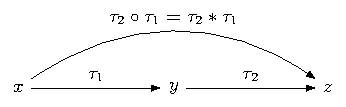
\includegraphics[width=0.82\textwidth]{../figures/composition.pdf}
\caption{Categorical layer. Morphisms are admissible traces, identities are empty traces, and composition is certified trace concatenation.}
\label{fig:composition}
\end{figure}

\section{Trace algebra}

\begin{theorem}[Telescoping law]
Let
\[
\tau:
x_0 \xrightarrow{\sigma_1} x_1 \xrightarrow{\sigma_2}\cdots \xrightarrow{\sigma_n} x_n
\]
be an admissible trace. Then
\[
V(x_n)+\sum_{i=1}^n s(\sigma_i)\le
V(x_0)+\sum_{i=1}^n d(\sigma_i).
\]
\end{theorem}

\begin{proof}
By induction on the trace length $n$.

For $n=1$, this is exactly the resource inequality in the definition of admissibility.

Assume the result holds for length $n$. Consider an admissible trace of length $n+1$:
\[
x_0 \xrightarrow{\sigma_1}\cdots \xrightarrow{\sigma_n} x_n \xrightarrow{\sigma_{n+1}} x_{n+1}.
\]
By the inductive hypothesis,
\[
V(x_n)+\sum_{i=1}^{n} s(\sigma_i)\le
V(x_0)+\sum_{i=1}^{n} d(\sigma_i).
\]
By admissibility of the final step,
\[
V(x_{n+1})+s(\sigma_{n+1})\le V(x_n)+d(\sigma_{n+1}).
\]
Combining the inequalities yields
\[
V(x_{n+1})+\sum_{i=1}^{n+1} s(\sigma_i)\le
V(x_0)+\sum_{i=1}^{n+1} d(\sigma_i).
\]
\end{proof}

\begin{corollary}
For an admissible trace, intermediate state valuations cancel from the aggregate resource bound.
\end{corollary}

\section{Semantic cost}

\begin{definition}[Verifier-realizable hidden traces]
For an observable trace $\tau$, let
\[
\Rset(\tau)
\]
denote the \emph{finite} set of verifier-realizable hidden traces projecting to $\tau$.
\end{definition}

\begin{definition}[Hidden trajectory cost]
Let
\[
W:\bigcup_{\tau}\Rset(\tau)\to \mathbb Q_{\ge 0}
\]
be a hidden trajectory cost.
\end{definition}

\begin{axiom}[Hidden cost subadditivity]
For composable verifier-realizable hidden traces,
\[
W(\Theta_2 * \Theta_1)\le W(\Theta_1)+W(\Theta_2).
\]
\end{axiom}

\begin{definition}[Semantic cost]
For an observable trace $\tau$, define
\[
s_{\semc}(\tau):=
\max_{\Theta\in \Rset(\tau)} W(\Theta).
\]
\end{definition}

\begin{remark}
The category uses the additive bookkeeping quantities
\[
s_{\syn},\ d_{\syn},
\]
while the semantic theorem below concerns the projected quantity
\[
s_{\semc}.
\]
This distinction is essential.
\end{remark}

\begin{theorem}[Subadditive semantic cost]
For admissible traces $\tau_1,\tau_2$ with compatible endpoints,
\[
s_{\semc}(\tau_2\circ\tau_1)
\le
s_{\semc}(\tau_1)+s_{\semc}(\tau_2).
\]
\end{theorem}

\begin{proof}
By definition,
\[
s_{\semc}(\tau_2\circ\tau_1)
=
\max_{\Theta\in\Rset(\tau_2 * \tau_1)} W(\Theta).
\]
Each hidden realization
\[
\Theta\in\Rset(\tau_2 * \tau_1)
\]
induces compatible restrictions
\[
\Theta_1\in\Rset(\tau_1),\qquad \Theta_2\in\Rset(\tau_2),
\]
and hence a restriction map
\[
\mathrm{res}:\Rset(\tau_2 * \tau_1)\to \Rset(\tau_1)\times \Rset(\tau_2).
\]
By hidden cost subadditivity,
\[
W(\Theta)\le W(\Theta_1)+W(\Theta_2).
\]
Taking maxima over the finite sets involved gives
\[
\max_{\Theta\in\Rset(\tau_2 * \tau_1)} W(\Theta)
\le
\max_{\Theta_1\in\Rset(\tau_1)} W(\Theta_1)
+
\max_{\Theta_2\in\Rset(\tau_2)} W(\Theta_2),
\]
which is exactly
\[
s_{\semc}(\tau_2\circ\tau_1)\le
s_{\semc}(\tau_1)+s_{\semc}(\tau_2).
\]
\end{proof}

\begin{figure}[t]
\centering
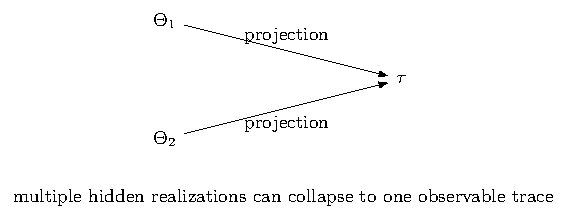
\includegraphics[width=0.72\textwidth]{../figures/projection.pdf}
\caption{Projection from hidden realizations to observables. Multiple hidden traces can collapse to the same observable trace, allowing semantic cost to differ from syntactic bookkeeping.}
\label{fig:projection}
\end{figure}

\section{Worked example: semantic cost strictly smaller than syntactic cost}

This example is designed to exhibit a genuine separation between syntactic bookkeeping and semantic realized cost.

\begin{definition}[Toy system]
Let
\[
X=\{A,B,C\},
\qquad
\Kadm=X.
\]

Let the hidden-state space be
\[
\Hid=\{A_0,A_1,B_0,C_0\},
\]
with projection
\[
\Pi(A_0)=A,\quad \Pi(A_1)=A,\quad \Pi(B_0)=B,\quad \Pi(C_0)=C.
\]
Thus
\[
\F_A=\{A_0,A_1\}
\]
contains two distinct hidden representatives of the same observable state.
\end{definition}

\begin{definition}[Valuation]
Set
\[
V(A)=5,\qquad V(B)=4,\qquad V(C)=3.
\]
\end{definition}

\begin{definition}[Payloads]
Take
\[
\Payload(A,B)=\{\alpha\},
\qquad
\Payload(B,C)=\{\beta\}.
\]
Let the corresponding control tokens be
\[
\kappa_{A,B}(\alpha)=t_\alpha,\qquad \kappa_{B,C}(\beta)=t_\beta.
\]
\end{definition}

\begin{definition}[Primitive steps]
Define
\[
\sigma_1:A\leadsto B,\qquad \sigma_2:B\leadsto C,
\]
with bookkeeping data
\[
s(\sigma_1)=1,\ d(\sigma_1)=0,
\qquad
s(\sigma_2)=1,\ d(\sigma_2)=0.
\]
\end{definition}

\begin{proposition}
Both primitive steps satisfy the resource inequality.
\end{proposition}

\begin{proof}
For $\sigma_1$:
\[
V(B)+s(\sigma_1)=4+1=5\le 5+0=V(A)+d(\sigma_1).
\]

For $\sigma_2$:
\[
V(C)+s(\sigma_2)=3+1=4\le 4+0=V(B)+d(\sigma_2).
\]
\end{proof}

Assume both steps are proposed and verifier-accepted. Let
\[
\tau:=\sigma_2 * \sigma_1.
\]

\begin{definition}[Composite hidden realization]
Assume
\[
\Rset(\tau)=\{\Theta^\star\}
\]
and
\[
W(\Theta^\star)=1.
\]
Intuitively, the composite admits hidden reuse or cancellation not visible in the syntactic bookkeeping.
\end{definition}

\begin{proposition}
For the composite trace $\tau$,
\[
s_{\syn}(\tau)=2,
\qquad
s_{\semc}(\tau)=1.
\]
In particular,
\[
s_{\semc}(\tau)<s_{\syn}(\tau).
\]
\end{proposition}

\begin{proof}
By additivity of syntactic bookkeeping,
\[
s_{\syn}(\tau)=s(\sigma_1)+s(\sigma_2)=1+1=2.
\]
Since $\Rset(\tau)=\{\Theta^\star\}$, the semantic cost is
\[
s_{\semc}(\tau)
=
\max_{\Theta\in \Rset(\tau)}W(\Theta)
=
W(\Theta^\star)
=
1.
\]
Hence
\[
s_{\semc}(\tau)<s_{\syn}(\tau).
\]
\end{proof}

\begin{figure}[t]
\centering
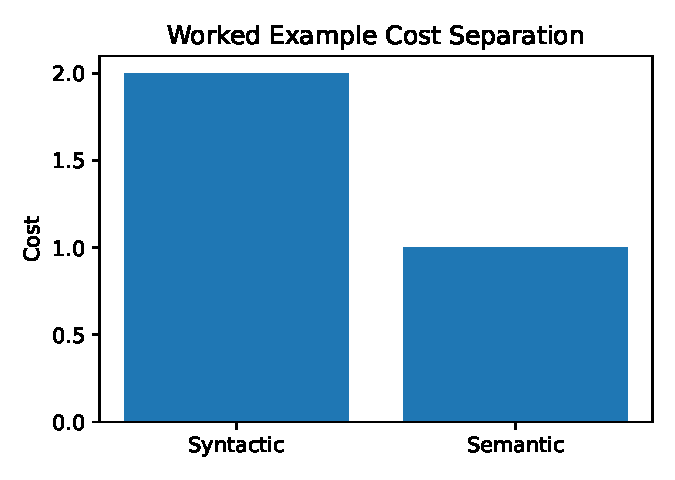
\includegraphics[width=0.62\textwidth]{../figures/cost_plot.pdf}
\caption{Worked example. Syntactic bookkeeping assigns cost $2$ to the composite trace, while semantic cost collapses to $1$ after projection through hidden realizations.}
\label{fig:cost}
\end{figure}

\begin{remark}
This example shows why the semantic layer is not reducible to bookkeeping. Projection can identify hidden realizations whose actual cost is strictly smaller than the visible syntactic total.
\end{remark}

\section{Positioning and scope}

The present paper makes a narrow foundational claim.

It is \emph{not} a complete general-purpose computation substrate. It is a formal categorical framework for verifier-certified execution traces with exact rational bookkeeping and a distinct semantic cost law induced by projection.

Its novelty lies in the order of construction:
\begin{itemize}[leftmargin=2em]
\item traces are first proposed,
\item then verified,
\item then admitted as morphisms.
\end{itemize}

Morphisms are therefore not assumed and decorated afterward; they are generated by admissibility.

\section{Conclusion}

We have defined a category whose morphisms are certified traces rather than freely given arrows. The category theorem depends explicitly on:
\begin{itemize}[leftmargin=2em]
\item exact rational numerics,
\item finite-valued admissible states,
\item a proposal mechanism,
\item a verifier closed under identity and concatenation,
\item additive syntactic bookkeeping.
\end{itemize}

We then separated syntactic cost from semantic cost and proved that projection from hidden realizations induces a subadditive semantic cost law.

Accordingly, the two main results of the paper are:

\[
\boxed{
\text{Certified traces form a category under concatenation.}
}
\]

\[
\boxed{
\text{Projection can strictly reduce semantic cost relative to syntactic cost.}
}
\]

This is the correct foundational claim.

\appendix

\section{Lean 4 formalization sketch}

The sketch below mirrors the paper's semantics more faithfully than placeholder traces of meaningless units. Each step carries a glyph with an explicit compiled control token and proof obligations.

\begin{verbatim}
inductive GlyphTag
| invoke
| bind
| route
| guard
| emit
deriving DecidableEq, Repr

structure ControlToken where
  opcode : String
  arg    : String
deriving DecidableEq, Repr

structure Glyph where
  tag         : GlyphTag
  surface     : String
  token       : ControlToken
  wf_surface  : Prop
  wf_token    : Prop

def Glyph.compiles (g : Glyph) : Prop :=
  g.wf_surface and g.wf_token

structure Step (X : Type) where
  src         : X
  dst         : X
  glyph       : Glyph
  costSpend   : Rat
  costDefect  : Rat
  typed       : Prop
  compiles_ok : glyph.compiles

structure Trace (X : Type) where
  steps : List (Step X)
  chain :
    forall  i : Nat, i + 1 < steps.length ->
      (steps.get ⟨i, Nat.lt_trans (Nat.lt_succ_self i) ‹i + 1 < steps.length›⟩).dst =
      (steps.get ⟨i+1, ‹i + 1 < steps.length›⟩).src

def traceSpend {X : Type} (t : Trace X) : Rat :=
  t.steps.foldl (fun acc s => acc + s.costSpend) 0

def traceDefect {X : Type} (t : Trace X) : Rat :=
  t.steps.foldl (fun acc s => acc + s.costDefect) 0

constant RVAccept : {X : Type} -> Trace X -> Prop

def emptyTrace {X : Type} (x : X) : Trace X :=
{ steps := [],
  chain := by
    intro i h
    cases Nat.not_lt_zero _ h }

def concat {X : Type} (t1 t2 : Trace X) : Trace X :=
{ steps := t1.steps ++ t2.steps,
  chain := by
    intro i h
    sorry }

structure CohMor (X : Type) (V : X -> Rat) (x y : X) where
  trace  : Trace X
  rv_ok  : RVAccept trace
  valid  : V y + traceSpend trace <= V x + traceDefect trace

axiom rv_id :
  forall {X : Type} (x : X), RVAccept (emptyTrace x)

axiom rv_comp :
  forall {X : Type} (t1 t2 : Trace X),
    RVAccept t1 -> RVAccept t2 -> RVAccept (concat t1 t2)
\end{verbatim}

\begin{remark}
A complete mechanization would refine the concatenation proof for \texttt{chain} and instantiate the glyph language with a concrete token semantics. The important point for the present paper is that the payload layer is no longer hidden behind \texttt{Type}: steps now carry explicit meaning objects, compiled control tokens, and proof obligations.
\end{remark}

\begin{thebibliography}{9}

\bibitem{kelly1982}
G. M. Kelly,
\textit{Basic Concepts of Enriched Category Theory},
Cambridge University Press, 1982.

\bibitem{lawvere1973}
F. W. Lawvere,
Metric spaces, generalized logic, and closed categories,
\textit{Rendiconti del Seminario Matematico e Fisico di Milano}, 43 (1973), 135--166.

\bibitem{benabou1967}
Jean B\'enabou,
\textit{Introduction to Bicategories},
Springer, 1967.

\bibitem{diaconescu1994}
Radu Diaconescu,
Category-based semantics for equational and constraint logic programming,
Technical Report PRG-116, Oxford University Computing Laboratory, 1994.

\bibitem{lambekscott1986}
Joachim Lambek and P. J. Scott,
\textit{Introduction to Higher Order Categorical Logic},
Cambridge University Press, 1986.

\end{thebibliography}

\end{document}
